% I'm not totally sure, if this should be described together or seperate, but somehow or SCRUM approach and the Redmine
% stuff should be mentioned somewhere before the developing part and as this are probably only three pages or somethin
% it probably could be integrated here
\chapter{Project Workflow and  Requirements}\label{chap:systemRequirements}

First of all, we've got a confession to make: Unplagged is like a big playground of new 
workflows and technologies for us, as we are aiming to incorporate 
\enquote{best-practices} wherever possible, or at least what we currently consider to be best-practices. 

We believe this approach is necessary, because of the 
fact, that we are essentially trying to incubate Unplagged as a real open source project and this will 
only work if
it is well crafted and if cutting-edge workflows and technologies are used. Nearly all of the team members
are also working in some kind of web related side job, so we all got enough experiences with the problems that can 
occur during the maintenance of badly designed software.

Most of the times this works pretty well, but sometimes we are still trying to figure out how to 
get everyone up to speed with every technology and part of the system or how to divide the responsibilites carefully.

To start this project, we opted to use \textit{Scrum} %\footnote{More information can be found at} 
as our agile development approach. If you are familiar with this
methodology, you may notice, that there could be a few problems when considering, that the team is working mostly 
distributed
without a common office and with very different time tables for each of the members.

We struggled a bit to the tweak the workflow that is required by Scrum in 

\section{The Workflow}

To make it possible to work efficiently together in this kind of environment, we chose to use
\href{http://www.redmine.org/}{Redmine} as our project management tool, which you can access under:

\begin{itemize}
\item \url{http://tickets.unplagged.com}
\end{itemize}

If you register there, an administrator should grant you access to the tickets and the wiki, so that you can participate
in solving the problems at hand.

% Redmine description, Meetings, Debbie, Scrum Cards, Server, Website


\subsection{Team Meetings}

\subsection{\enquote{Debbie Meetings}}

\begin{figure}[!h]
  \centering
    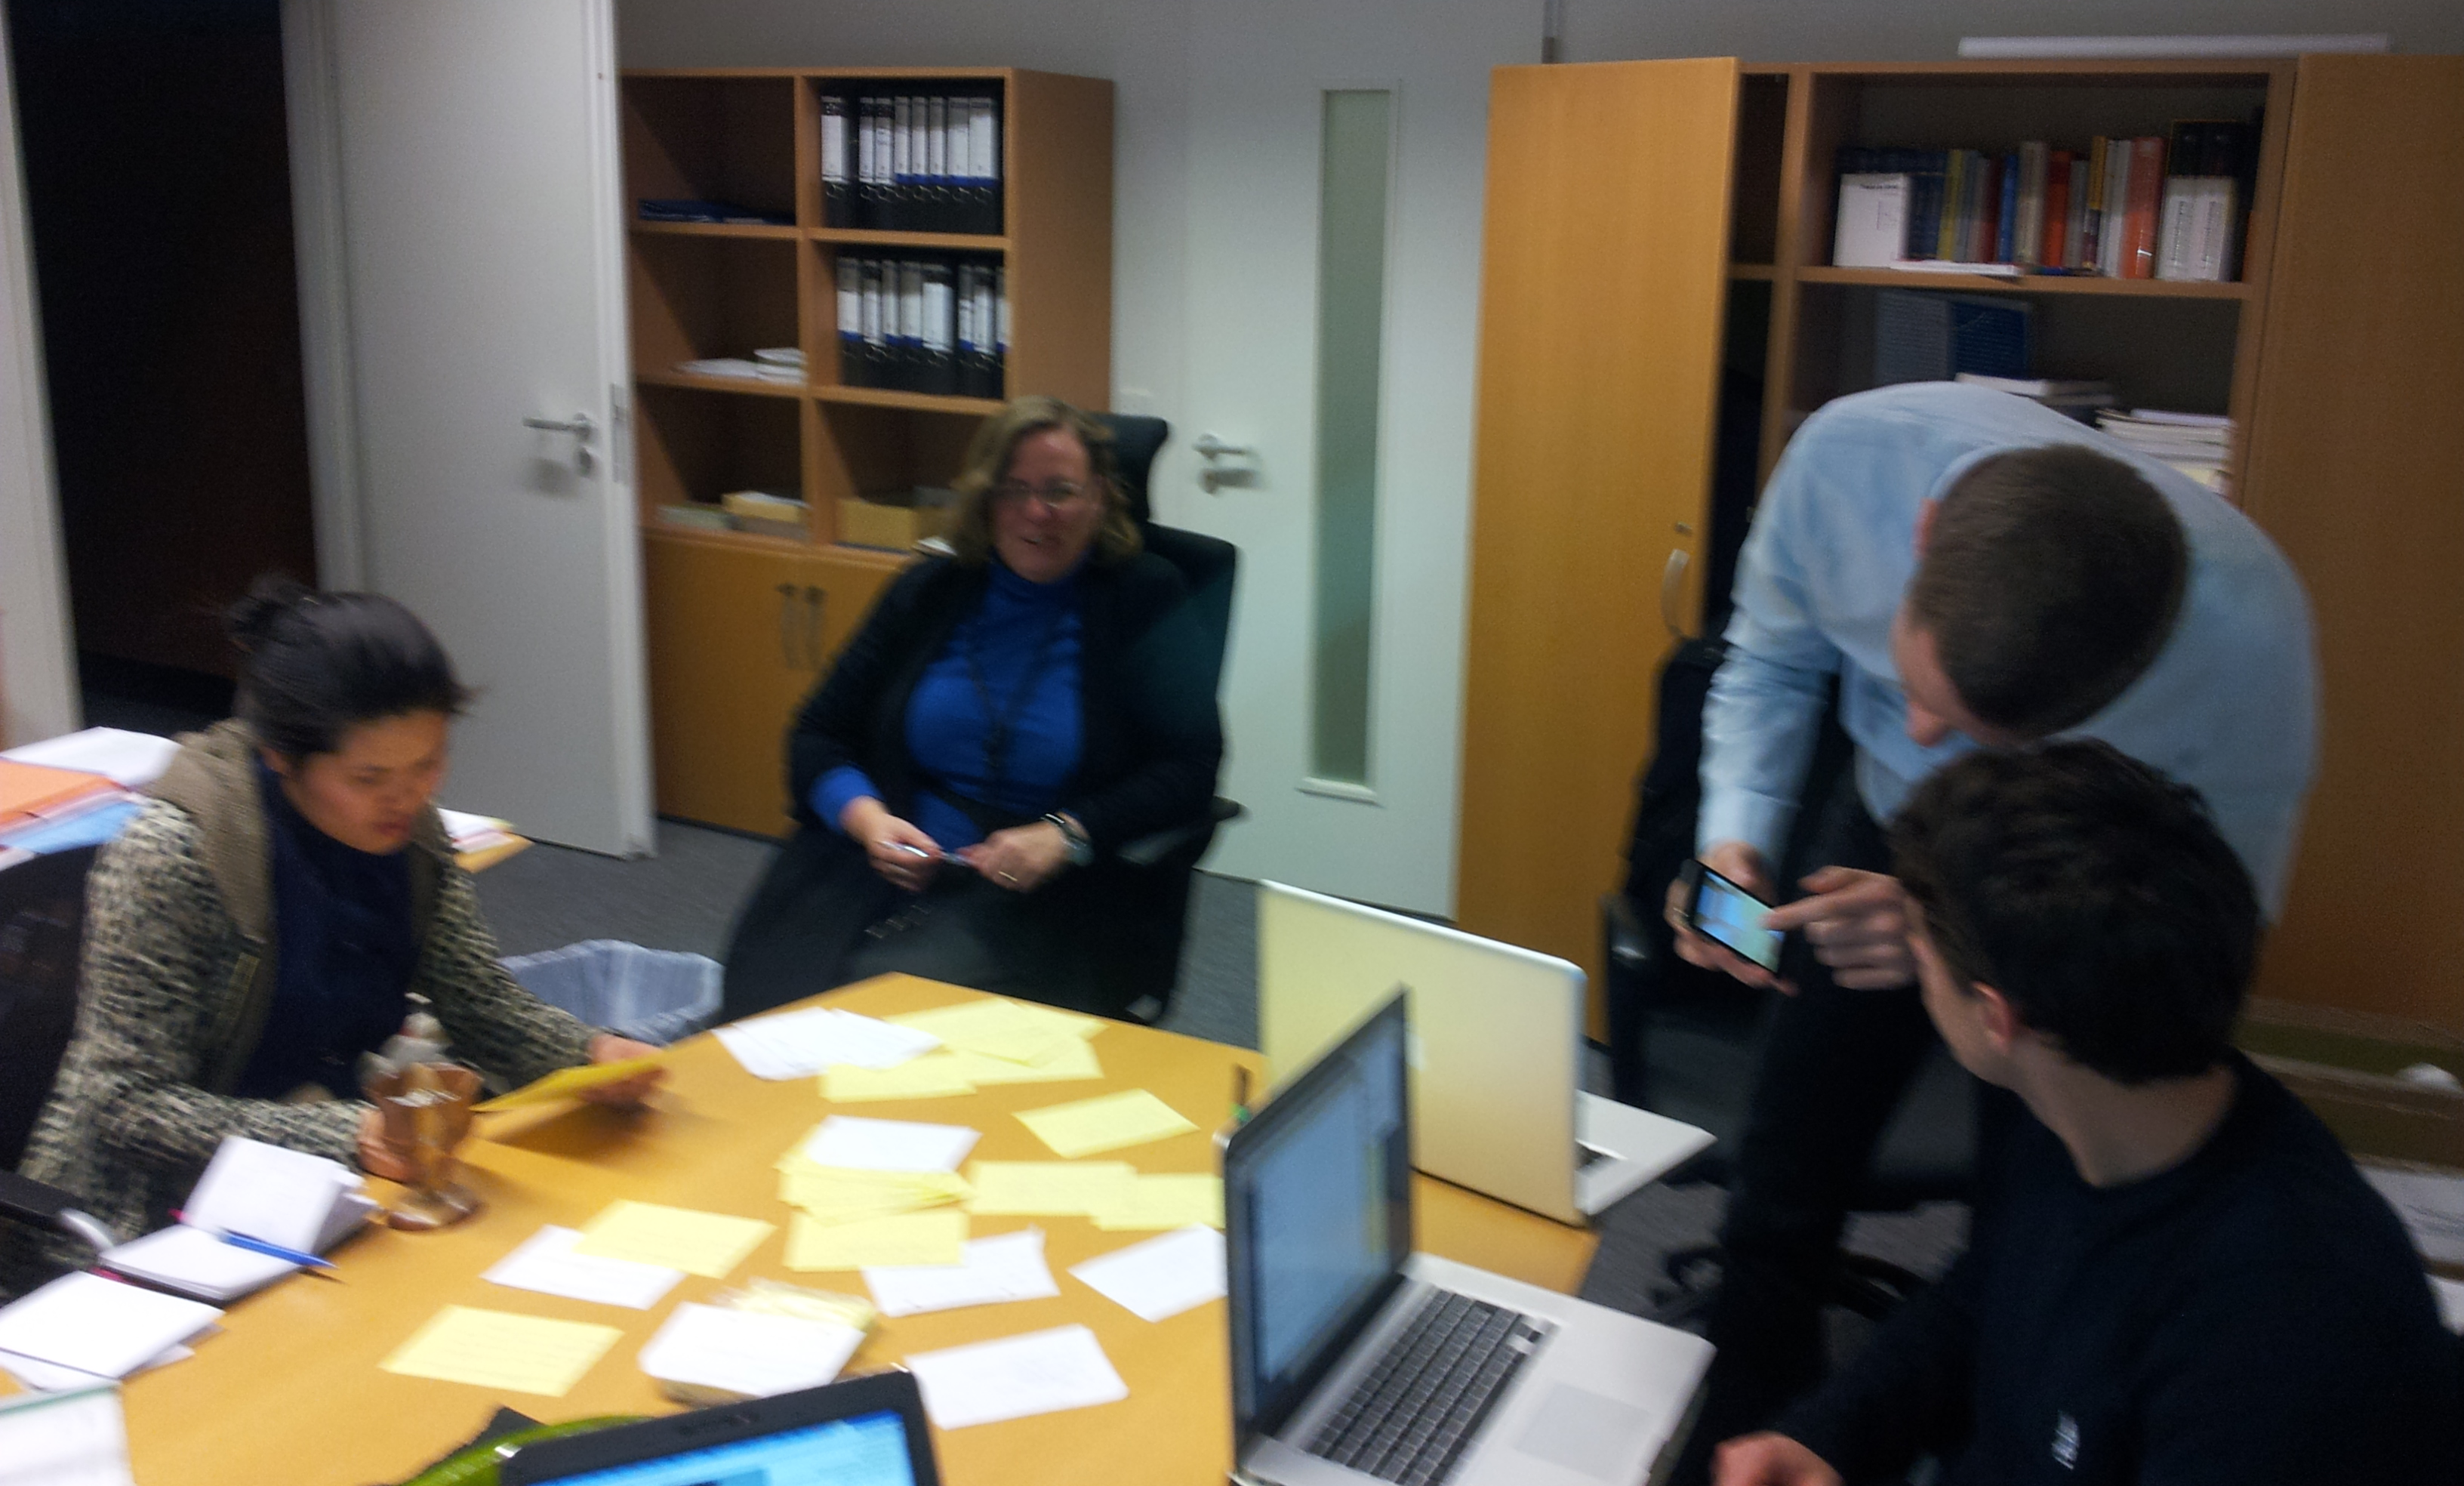
\includegraphics[width=0.8\textwidth]{images/2011-11-15-user-stories-6.jpg}
  \caption{Scrum Meeting}
  \label{fig:scrumming}
\end{figure}

\begin{figure}[!h]
  \centering
    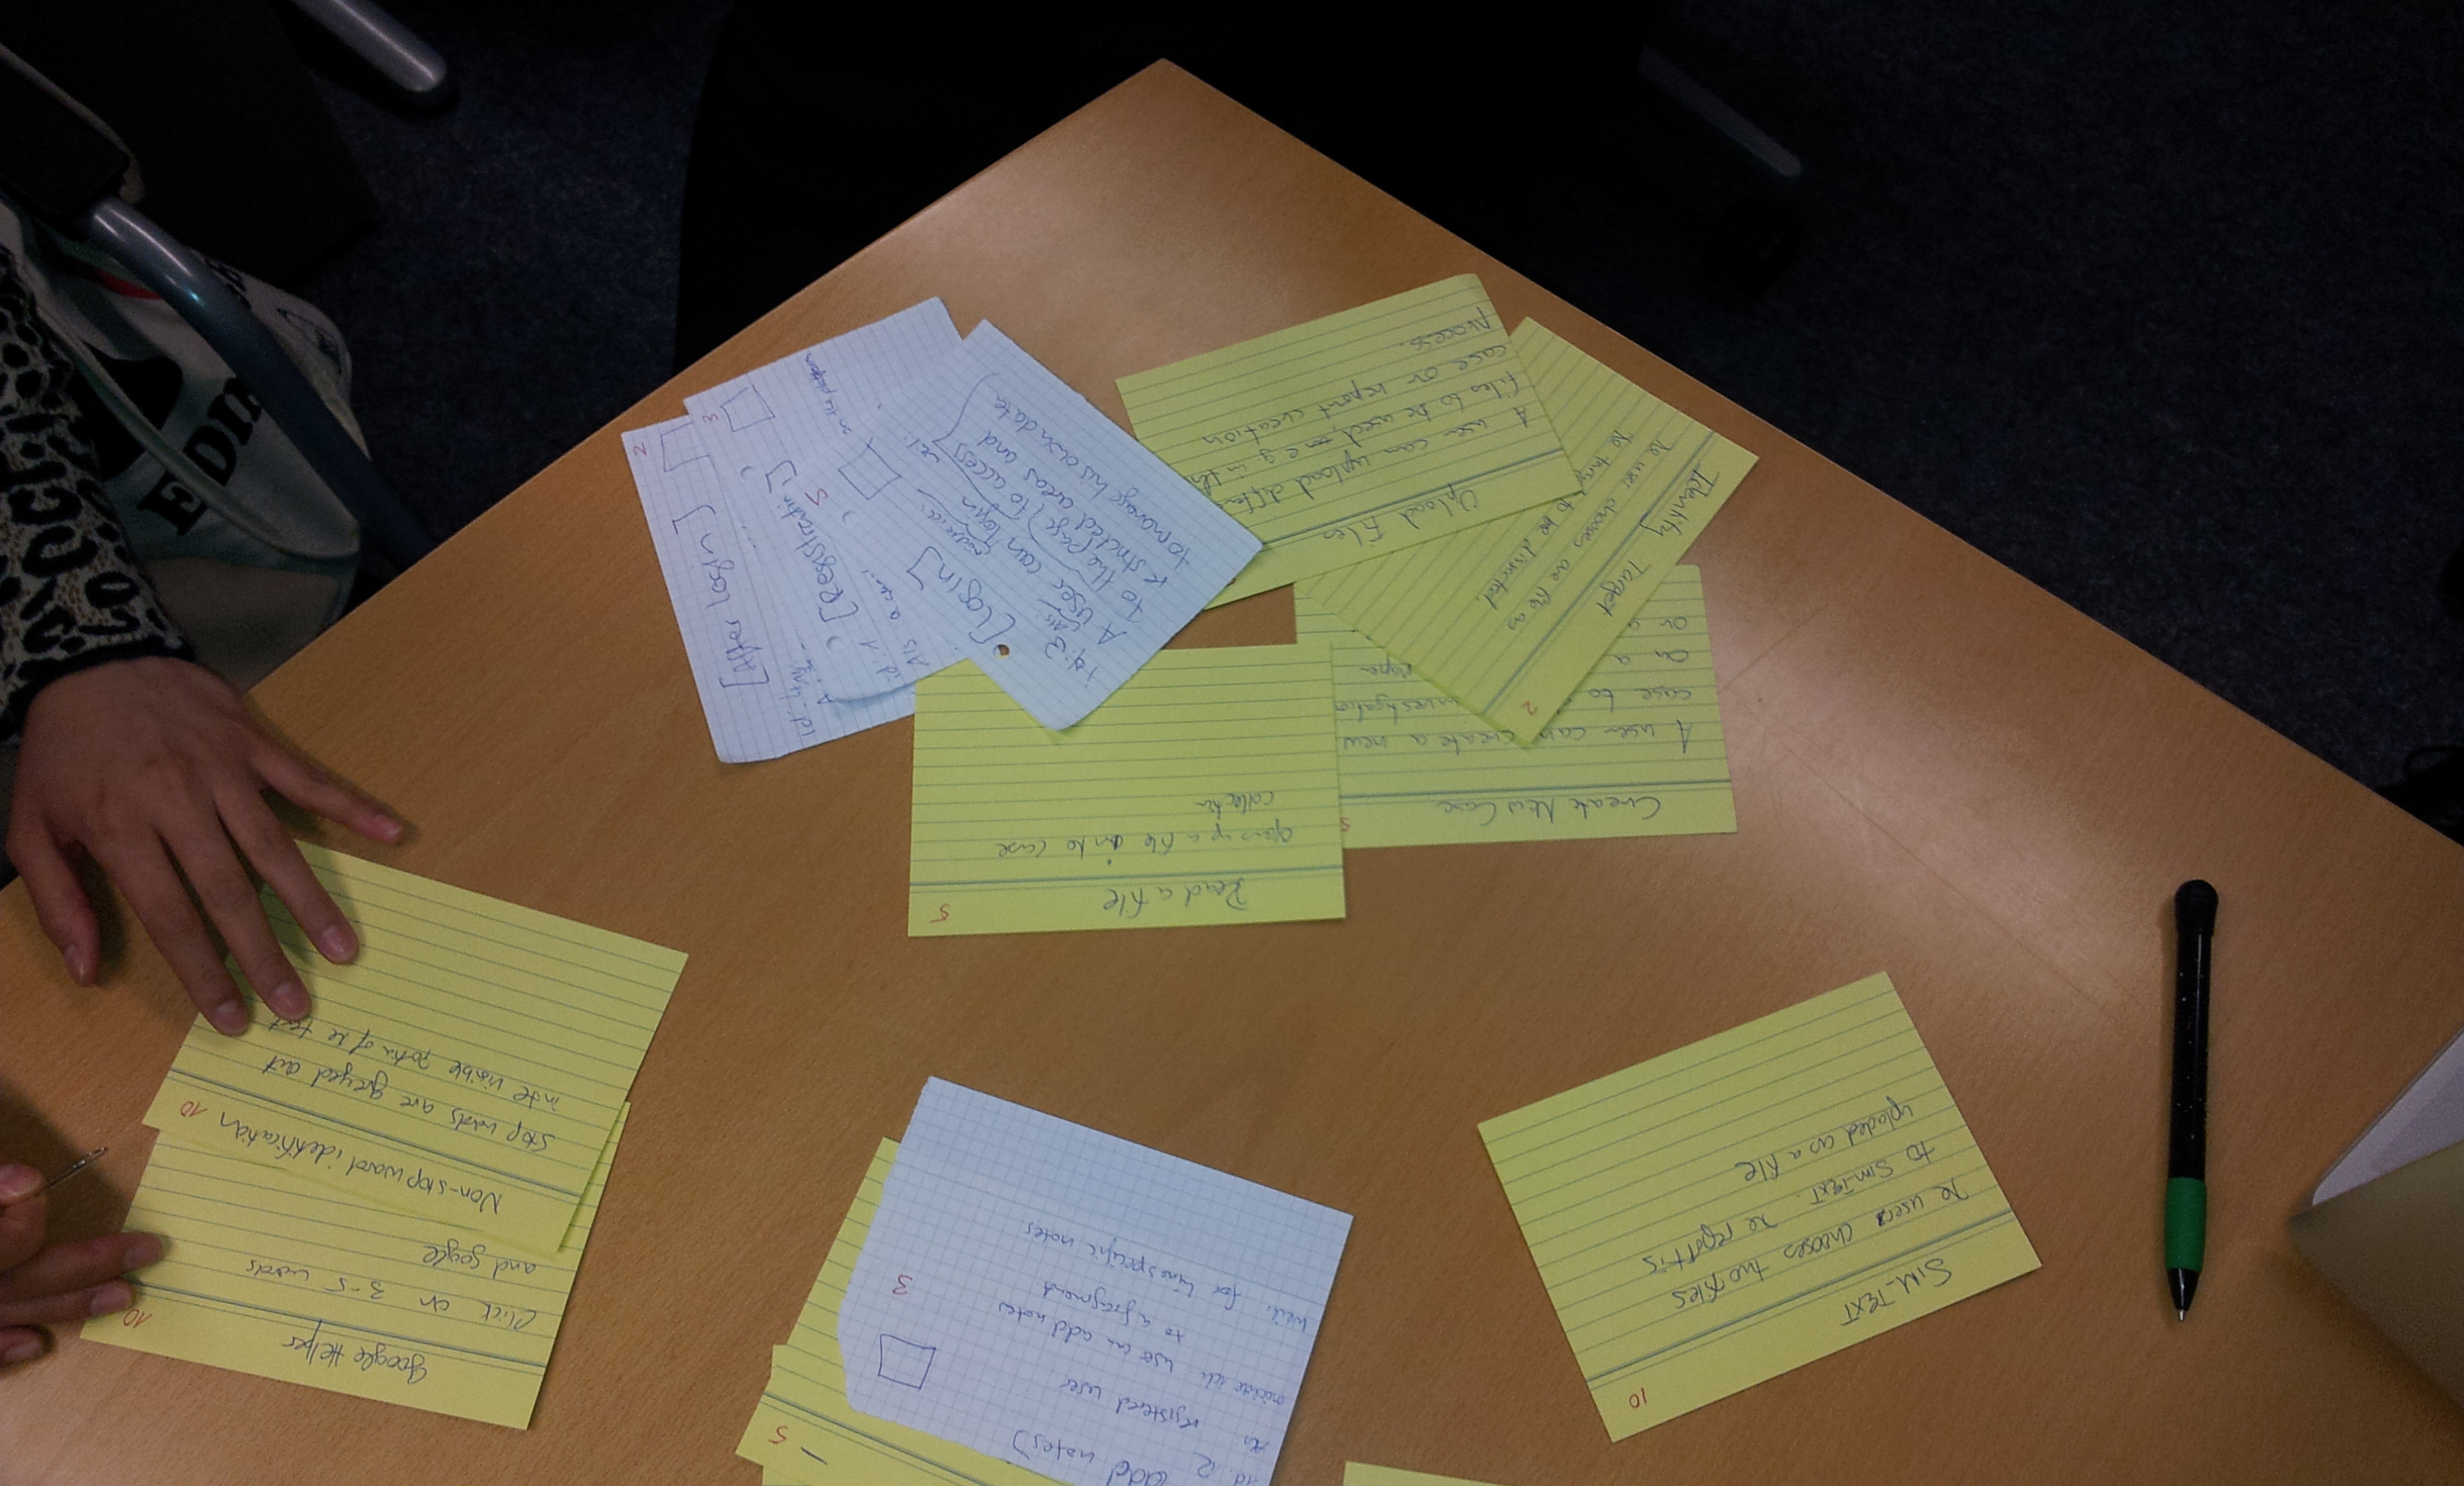
\includegraphics[width=0.8\textwidth]{images/2011-11-15-user-stories-4.jpg}
  \caption{User Stories}
  \label{fig:userStories}
\end{figure}

\section{Target Group}

\section{User roles}

As the Unplagged system will provide a permission based user system, our goal is to make it possible, to create custom user roles from an administration area and make it possible for users to have multiple user roles in one case and also different roles for different cases.
The standard roles which will be provided by the system are:

\begin{description}
\item[Guest]
A user without a valid login can only see the parts of cases that are set to be public.
\item[Registered]
Registered users can get \enquote{promoted} to higher roles and contribute to publicly editable cases.
%Note: Do we want users to register themselves? Or do we have just an admin, that takes care of this? I'm currently also not sure if this will really need to be a role, or if Guest and Registerd are just two basic states.
\item[Collaborator]
Collaborators are registered users who were granted access to a specific case. Collaborators can access and edit these projects.
\item[Case-Manager]
Case-Managers can set up new cases and manage colloborators for their cases and project versions. They may have the permission to add or remmove project members.
%Note: What does manage project versions mean?
\item[Admin]
An admin owns all permissions, such as user administration or project administration. They also hvae the ability to to block/unblock an existing case.
\end{description}

\section{Basic functionalities}

\section{Document Parser}

\section{Detection Modes}

\section{Plugin Architecture}

%Perhaps better on the way for every part?
\section{Use Cases}
